% ══════════════════════════════════════════════════════════
\section{Architecture}

The application follows the \textbf{Model--View--ViewModel (MVVM)} pattern with manual dependency injection (no DI framework).

\subsection{Layer Diagram}

\begin{figure}[H]
  \centering
  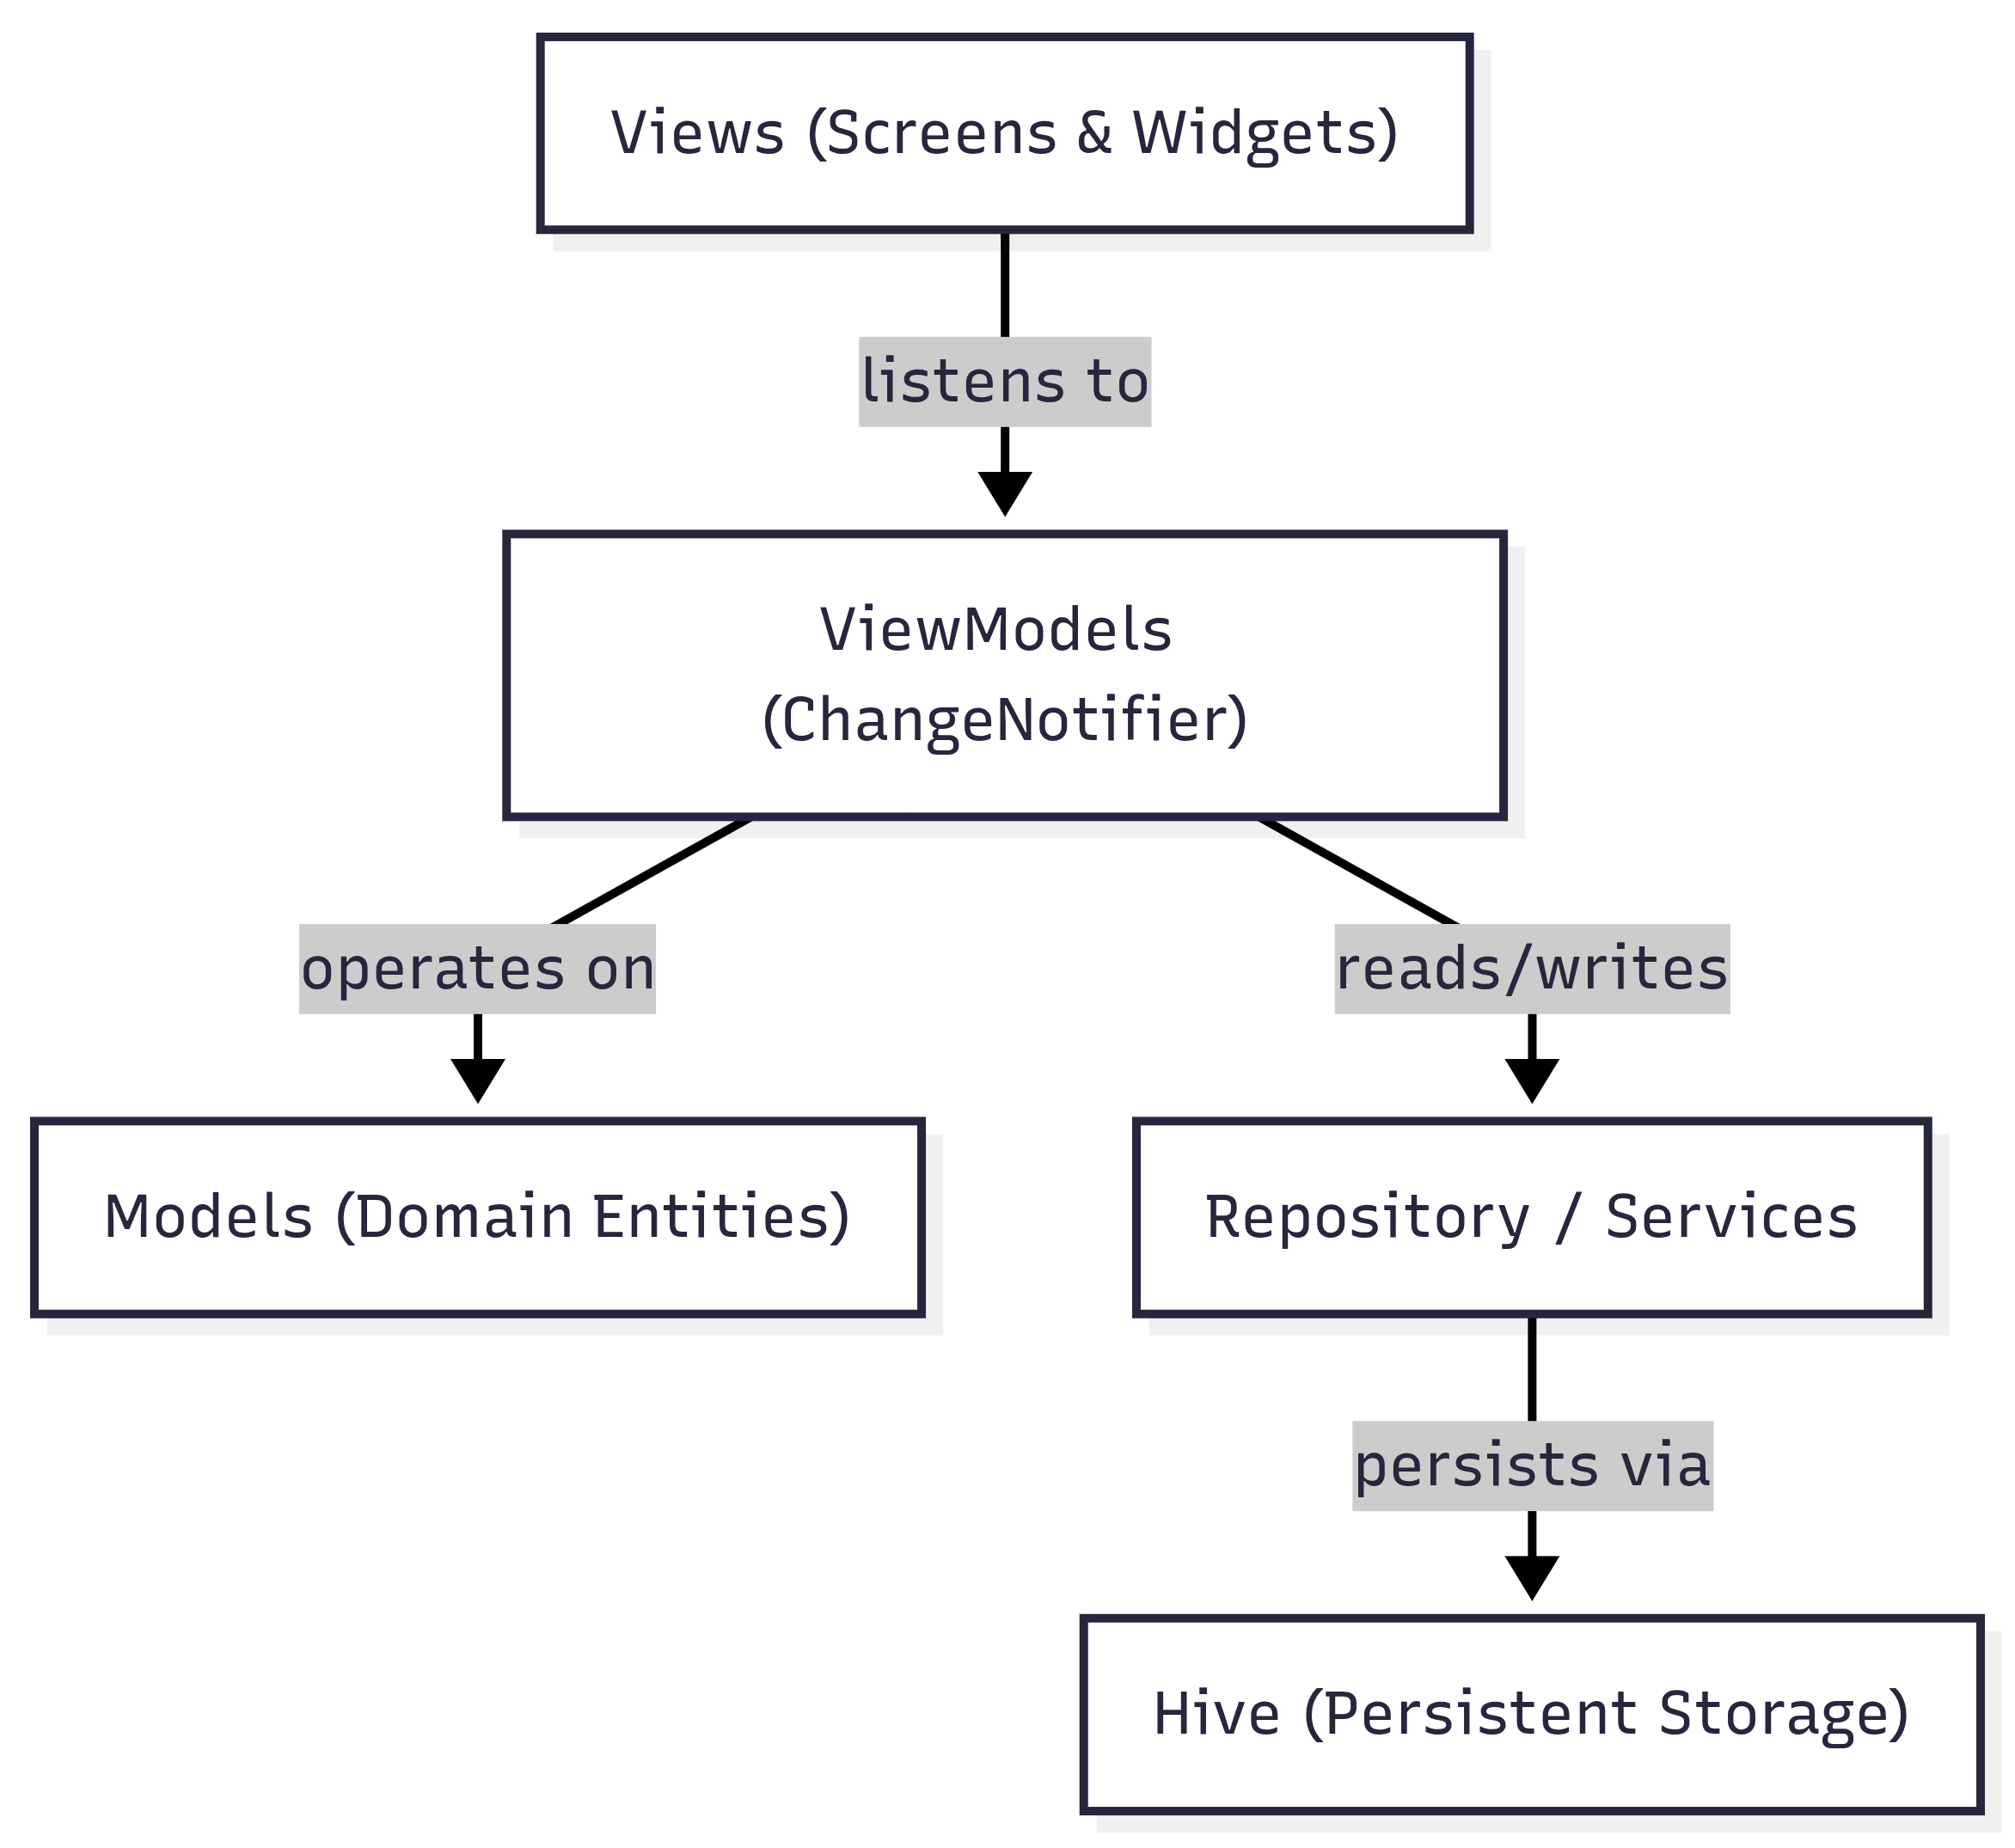
\includegraphics[width=0.7\textwidth]{images/layer-diagram.png}
  \caption{Layer Diagram}
\end{figure}

\subsection{Layer Responsibilities}

\begin{description}[style=nextline]
  \item[Models (\texttt{lib/models/})]
    Pure Dart domain entities with no framework dependencies. Business logic lives in entity methods (e.g.\ \texttt{Order.calculatePointsEarned()}, \texttt{CartItem.calculateSubtotal()}). Constructors use \texttt{assert} for invariant validation.

  \item[ViewModels (\texttt{lib/viewmodels/})]
    State holders extending \texttt{ChangeNotifier}. Each screen has a corresponding ViewModel that manages its state and exposes methods for user actions. ViewModels are manually wired in \texttt{main.dart} and passed as constructor parameters.

  \item[Views (\texttt{lib/views/})]
    \texttt{StatelessWidget} screens that receive their ViewModel via constructor injection. Navigation uses raw \texttt{Navigator.push}.

  \item[Repository (\texttt{lib/repositories/})]
    \texttt{AppRepository} aggregates all ViewModels and coordinates cross-cutting concerns (e.g.\ awarding stamps and points after checkout).

  \item[Services (\texttt{lib/services/})]
    \texttt{LocalStorage} wraps \texttt{Hive} for persisting user profile data, orders, cart items, and loyalty stamp count.
\end{description}
